\documentclass[tikz]{standalone}
\usetikzlibrary{arrows}
\begin{document}
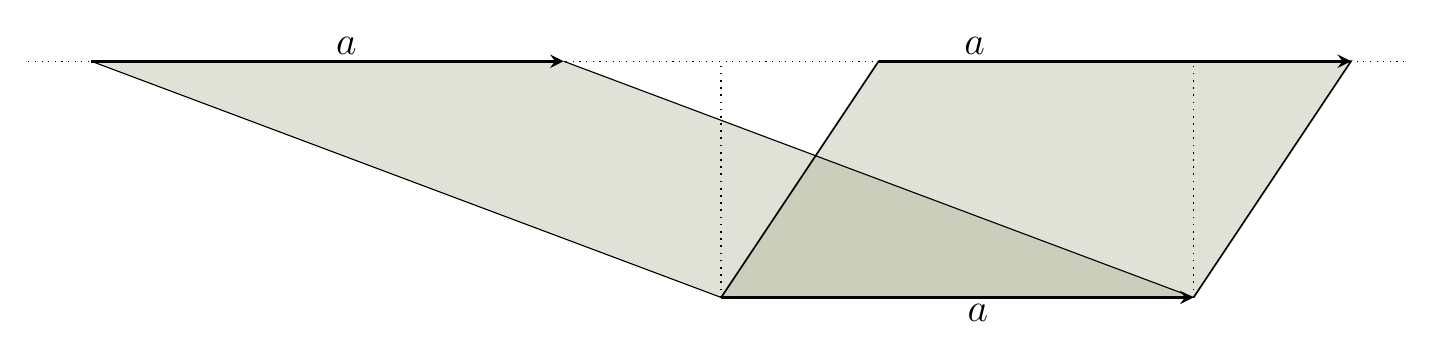
\begin{tikzpicture}[scale=1.0]
% ------------------------------------------------ lin_alg theme colors
\definecolor{la_white}{RGB}{233,235,223} %#E9EBDF
\definecolor{la_dark}{RGB}{59,54,81}     %#3B3651
\definecolor{la_gray}{RGB}{96,112,139}   %#60708B
\definecolor{la_tan}{RGB}{152,159,122}   %#989F7A


%\fill[line width=0.6pt,color=la_gray,fill=la_gray,fill opacity=0.5] (0,0) -- (6,0) -- (6,3) -- (0,3) -- cycle;

\fill[line width=0.6pt,color=la_tan,fill=la_tan,fill opacity=0.3] (2,3) -- (0,0) -- (6,0) -- (8,3) -- cycle;
\fill[line width=0.6pt,color=la_tan,fill=la_tan,fill opacity=0.3] (-8,3) -- (0,0) -- (6,0) -- (-2,3) -- cycle;

%\draw [line width=0.6pt,color=black] (0,0)-- (6,0) -- (6,3) -- (0,3) -- (0,0);
\draw [line width=0.6pt,color=black] (6,0)-- (8,3) -- (2,3) -- (0,0);

\draw [line width=0.6pt,dotted,color=black] (0,0)-- (0,3);
\draw [line width=0.6pt,dotted,color=black] (6,0)-- (6,3);

\draw [line width=0.4pt,dotted,domain=-8.8:8.74] plot(\x,{(--12-0*\x)/4});

\draw [color=black] (-8,3)-- (0,0);
\draw [color=black] (6,0)-- (-2,3);

% ---------------------------------------------  Vectors and Vector Labels
\draw [line width=0.4mm,>=stealth,->] (-8,3) -- (-2,3);
\draw [line width=0.4mm,>=stealth,->] (2,3) -- (8,3);
\draw [line width=0.4mm,>=stealth,->] (0,0) -- (6,0);

\draw[color=black] (-4.76,3.2) node {\Large $a$};
\draw[color=black] (3.22,3.2)  node {\Large $a$};
\draw[color=black] (3.26,-0.2) node {\Large $a$};

\end{tikzpicture}
\end{document}